Das Raspberry Pi ist das zentrale Element des Systems. Das Pi ist nichts anderes als ein Mini-Computer. Ergänzt wird das Pi mit einem WLAN-Adapter, damit die drahtlose Kommunikation gewährleistet werden kann. \\
\\
Der Mini-Computer ist wie folgt ausgestattet (Modell B+):
\begin{itemize}
	\item CPU: 700Mhz Broadcom BCM2835
	\item RAM: 512 MB
	\item 4 USB Ports
	\item 40pin extendeded GPIO
	\item Full size HDMI
	\item Micro SD Slot (mit 8GB Micro SD)
	\item CSI Schnittstelle
\end{itemize}

Das Pi kann grundsätzlich zu viel. Die CPU und RAM sind für heutige Verhältnisse nicht gerade berauschend, jedoch genügend für unsere Anforderungen. Im Notfall können ressourcenintensive Berechnungen auf die externe Steuerungseinheit ausgelagert werden. Ein USB Port wird durch den WLAN-Adapter besetzt. Über die GPIOs wird das Freedom-Board verbunden. Die CSI-Schnittstelle dient dazu die PI Camera anzuhängen \cite{raspberri-b-plus-spec}.\\
\\
Auf der SD Karte wird das Betriebssystem Arch Linux installiert. Diese Linux-Distribution ist minimalistisch ausgestattet. Es braucht lediglich 64 MB Ram und weniger als 800 MB Speicherplatz. So können die Hardware-Ressourcen, welche begrenzt sind, für das wirklich wichtige eingesetzt werden \cite{arch-linux-system-requirements}.

\begin{figure}[h!]
	\centering
	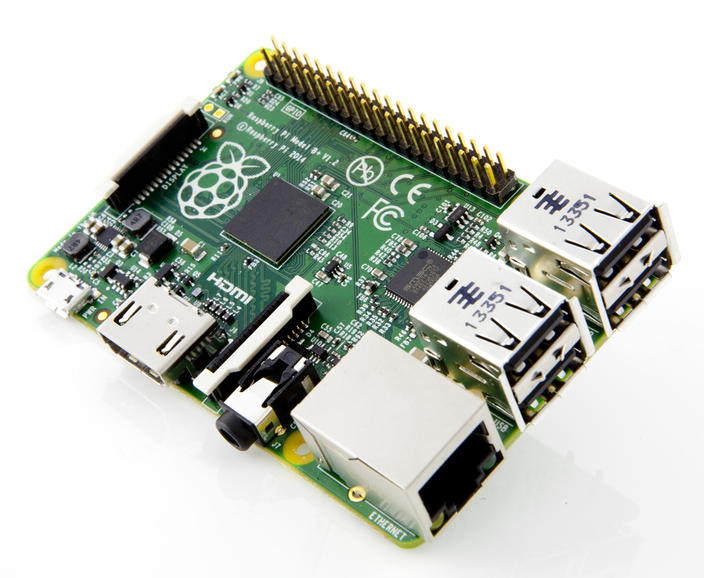
\includegraphics[width=0.3\linewidth]{../../fig/raspberry-pi-b-plus.jpg}
	\caption{Raspberry Pi B+}
	\label{fig:raspberry-pi-b-plus}
\end{figure}
